\section{Modul Web}

V~tomto modulu implementujeme webovou aplikaci, která zpřístupňuje naši knihovnu, pro výpočet dostupnosti, běžným uživatelům. Součástí tohoto modulu je také implementace interaktivní vizualizace, popsané dříve v~sekci~\ref{Interaktivni-vizualizace}.

\subsection{Části webové aplikace}

Před samotným popisem modulu si popíšeme části webové aplikace, které budeme implementovat.

Hlavní stránkou webové aplikace je stránka \textbf{Finder}, skrze níž mohou uživatelé vyhledávat dostupnost, viz obrázek~\ref{fig:Finder}.

\begin{figure}[ht]
    \centering
    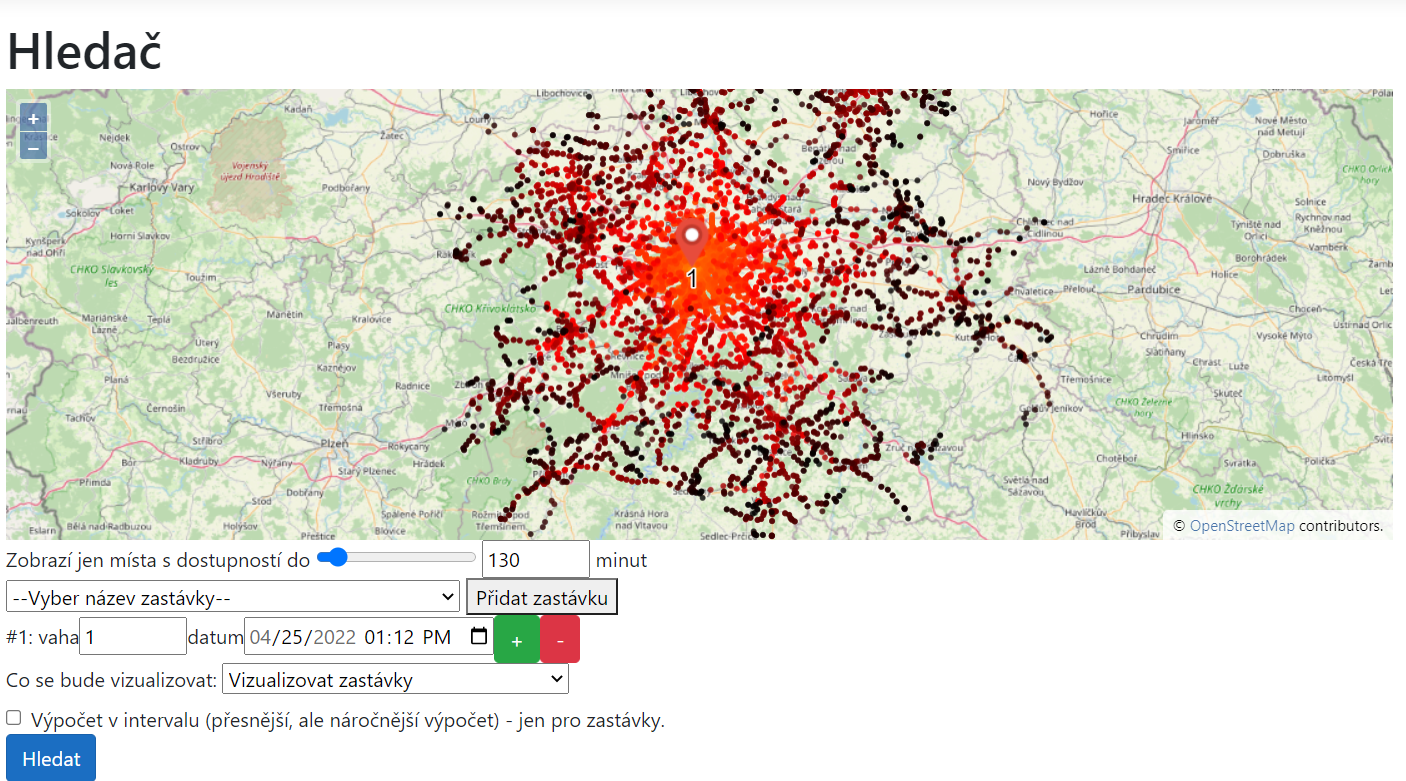
\includegraphics[width=\textwidth]{../img/finder.png}
    \caption{Stránka Finder.}
    \label{fig:Finder}
\end{figure}

\subsubsection{Značky}
% mozna pridat obrazek ikony markeru se zdrojem

Přidání značky reprezentující vstupní místo je možné dvěma způsoby. Kliknutím do mapy, nebo výběrem zastávky ze seznamu všech zastávek.

Vybrané vstupní místo lze odstranit kliknutím na značku asociovanou k~tomuto místu.

Značky lze po mapě přesouvat myší.

\subsubsection{Formulář se vstupními místy}

Formulář se vstupními místy generujeme dynamicky. Pro každé nové vstupní místo přidáváme položku.

S~každým vstupním místem asociujeme váhu a~skupinu dat s~časy. Váhu používáme k~výpočtu váženého průměru. Data s~časy určují dobu, kdy ze zastávky chceme vyjíždět. Data s~časy lze přidávat tlačítkem $+$ a~odebírat tlačítkem $-$.

Vizualizovat můžeme zastávky, body nebo obojí.

Při vizualizaci zastávek vizualizujeme všechny zastávky, které dostupné ze vstupních míst.

Při vizualizaci bodů vytváříme čtvercový rastr o~rozlišení daném konstantou \textbf{VisualisedRasterPointsResolution}, viz sekce~\ref{optim-body}. Mezi vizualizovanými body jsou jen ty, které jsou v~maximální vzdálenosti, dané konstantou \textbf{NearestStopsDistanceInMeters}, od nejbližší dostupné zastávky. Konstanty pochází z~konfiguračního souboru.

Uživatel si může zažádat o~výpočet v~intervalu, viz metoda \textbf{CalcAccessibility} v~sekci~\ref{Metoda-CalcAccessibility}. Takový výpočet je náročnější než klasický výpočet, jeho výsledky jsou však přesnější.

Formulář lze odeslat ke zpracování kliknutím na tlačítko \textbf{Hledat}. Po vypočtení dostupnosti dojde k~vizualizaci bodů na mapě.

Pokud byla některá značka na místě vzdáleném o~více než \textbf{NearestStops\hyp{}DistanceInMeters} od nejbližší zastávky, dojde k~vypsání chyby a~označení vstupního místa způsobujícího chybu, viz obrázek~\ref{fig:Finder-chyba}.

\begin{figure}[ht]
    \centering
    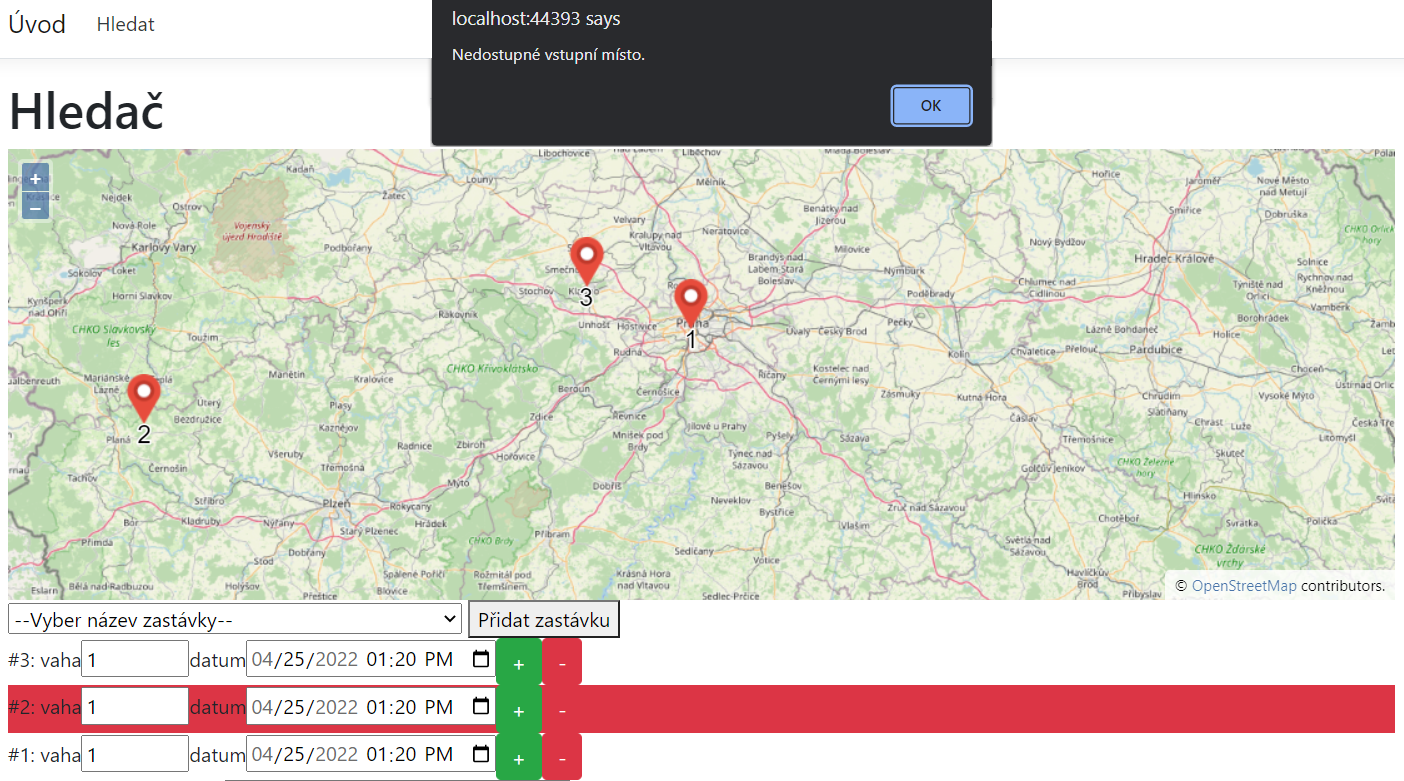
\includegraphics[width=\textwidth]{../img/finder-chyba.png}
    \caption{Hlášení chyby při zadání nedostupného místa.}
    \label{fig:Finder-chyba}
\end{figure}

\subsubsection{Výsledná dostupnost}

Dostupnost na vizualizovaných místech barevně rozlišujeme. Tmavě jsou označena méně dostupná místa a~světle jsou označena dostupnější místa.

Pro snazší hledání dostupných míst jsme zavedli posuvník, kterým lze omezit maximální vizualizovanou dostupnost. Barvy na vizualizovaných místech překreslujeme v~závislosti na aktuálně nastavené maximální dostupnosti.

Nejdostupnější místa vypisujeme v~tabulce pod formulářem.


\subsection{Backend}

Náš backend je postavený nad webovým frameworkem ASP.NET Core. Framework ASP.NET jsme zvolili, neboť naše knihovní část je napsaná v~jazyku C\# a~ASP.NET je velice populárním frameworkem pro tento programovací jazyk.

\subsubsection{Volba modelu}

Framework ASP.NET umožňuje vytvářet webové aplikace ve dvou modelech, \textbf{ASP.NET MVC} a~\textbf{Razor Pages}.

\begin{itemize}
    \item \textbf{ASP.NET MVC} je postavený na návrhovém vzoru Model–view–controller, který odděluje UI, data a~logiku. Použití tohoto návrhového vzoru sice zvyšuje flexibilitu, cenou je však vyšší složitost. Důsledkem těchto vlastností je tento model vhodný spíše pro větší aplikace.
    \item Model \textbf{Razor Pages} je jednodušší, odděluje pouze UI a~logiku.
\end{itemize}

My jsme zvolili model \textbf{Razor Pages}, neboť naše aplikace není příliš rozsáhlá a~MVC by nám do aplikace zanášelo zbytečnou složitost.

\subsubsection{Zpřístupnění knihovny jako Dependency Injection služby}

Abychom mohli využívat námi implementovanou knihovnu pro výpočet dostupnosti, musíme ji nejprve zpřístupnit pro webovou aplikaci.

Toho docílíme načtením potřebných modulů jako služby. Načítání služby obstarává metoda \textbf{ConfigureServices} uvnitř třídy \textbf{Startup}. Každá služba má přiřazenou životnost, my používáme typy životnosti \textbf{singleton} a~\textbf{scoped}.

\begin{itemize}
    \item \textbf{Singleton} --- existuje jedna instance pro všechny webové dotazy.
    \item \textbf{Scoped} --- existuje nová instance pro každý webový dotaz.
\end{itemize}

Načtené služby jsou nám následně zpřístupněny za pomoci \textbf{Dependency Injection} skrze konstruktor.

\subsubsection{Stránka Finder}

\textbf{Finder} je hlavní stránka naší webové aplikace.

Metodu \textbf{OnPost} využíváme ke zpracování vstupu, zadaného uživatelem do formuláře.

Jelikož počet vstupních zastávek zadaných uživatelem není předem známý, potřebujeme data získávat z~dynamicky rozšiřitelného formuláře. To bohužel znemožňuje použití \textbf{bindování}, které ASP.NET poskytuje pro uložení uživatelského vstupu přímo do atributů. Místo toho použijeme pro přenos dat formát \textbf{JSON} (JavaScript object notation).

Pro vizualizaci bodů potřebujeme znát sousedy těchto bodů. Tyto sousedy si můžeme vyhledat jednou a~pracovat s~nimi v~dalších výpočtech, viz sekce~\ref{optim-body}. Toto je implementováno ve třídě \textbf{PointsWithNeighbors}.

\subsubsection{Třída DataUpdater}\label{trida-DataUpdater}

Třída \textbf{DataUpdater} zajišťuje aktualizaci dat jízdních řádů.

Metoda \textbf{GetTimetable} poskytuje přístup k~instaci třídy \textbf{Timetable}, popsané v~sekci~\ref{class-timetable}.

K~aktualizaci dat dojde v~případě, že je nastavený \textbf{ShouldUpdate} v~konfiguračním souboru nebo pokud chybí serializace dat jízdních řádů.

Během aktualizace stahujeme zazipovaná data z~adresy dané konstantou \textbf{GTFSSourceURI} a~následně je extrahujeme do složky na cestě dané konstantou \textbf{PathToGTFSFolder}. Konstanty pochází z~konfiguračního souboru.

\subsubsection{Možné zlepšení}

Pokud bychom chtěli kromě webové aplikace vytvářet také mobilní či desktopovou aplikaci, mohli bychom využít ASP.NET Web API, které umožňuje vytváření \textbf{REST API}. Tento přístup jsme nevyužili, neboť bychom vedle samotného Web API museli vytvářet ještě samotnou webovou aplikaci a~to by do naší aplikace zanášelo další složitost.


\subsection{Frontend}

Jako programovací jazyk pro frontend jsme zvolili populární \textbf{JavaScript}. Interaktivní mapu vytváříme s~pomocí knihovny \textbf{OpenLayers}. Ke stylování HTML prvků používáme knihovnu \textbf{Bootstrap 4}.

Všechen JavaScriptový kód pro stránku \textbf{Finder} se nachází v~souboru \textbf{map.js}. Vedle pomocných funkcí a~konstant jsou v~souboru obsaženy dvě hlavní třídy, \textbf{Form} a~\textbf{OLMap}.


\subsubsection{Třída Form}

Tato třída obsahuje metody pro práci s~formulářem, do kterého uživatel zadává vstupní místa.

Formulář je dynamický, díky čemuž můžeme za běhu přidávat vstupní místa, případně data s~časy asociované se vstupními místy. To zajišťují metody \textbf{addField} a~\textbf{removeField}.

Data z~formuláře odesíláme na server ve formátu \textbf{JSON}. Zpracování dat a~jejich \textbf{serializaci} obstarává metoda \textbf{submit}. Odpověd ze serveru je také zpracovaná touto metodou. V~případě, že uživatel zadal nedosažitelné vstupní místo, volá se metoda \textbf{unreachableTargetHandler}. Pokud vše proběhlo v~pořádku, vrátí se nám ze serveru dostupnost pro všechny zastávky či místa, s~tou dále pracujeme v~metodě \textbf{handleResponse}.

Framework ASP.NET obsahuje ochranu proti CSRF (Cross-Site Request Forgery) útokům pomocí tokenu \textbf{\_\_RequestVerificationToken} vloženého do fomuláře jako hidden field. Abychom umožnili posílání dat z~JavaScriptu na server, musíme s~nimi posílat také tento token.


\subsubsection{Třída OLMap}

V~této třídě vytváříme interaktivní mapu pomocí knihovny \textbf{OpenLayers}.

V~konstruktoru skládáme mapu z~vrstev. \textbf{TileLayer} obsahuje mapy z~OSM. \textbf{MarkerLayer} slouží pro zobrazení značek, které uživatel umísťuje do mapy. \textbf{VisualizationLayer} slouží k~zobrazeni bodů s~barvou v~závislosti na jejich dostupnosti.

V~konstruktoru dále nastavujeme funkcionalitu potřebnou pro přesouvání značek umístěných v~mapě. Logiku pro přesouvání značek zajišťují metody \textbf{updateFormOnMarkerMovement} a~\textbf{changeCursorOnMarkerMovement}.  

Třída dále obsahuje metodu \textbf{addOrRemoveMarker}, která reaguje na kliknutí do mapy a~umožňuje tak přidávání a~odebírání značek.

\subsubsection{Možné vylepšení}

Přestože naše knihovna dokáže vypočítat dostupnost pro zcela libovolné místo, naše webová aplikace to uživatelům neumožňuje. Webová aplikace umožňuje jen vyhodnocení dostupnosti v~předem daných bodech a~na zastávkách.

Pro uživatele by mohlo být zajímavé řešení, které by zobrazovalo dostupnost pro místo na které ukazuje kurzor myši.

Pokud bychom posílali dotaz pro výpočet dostupnosti při každém pohybu myši, nejspíše by došlo snadno k~zahlcení serveru. Ideální by bylo provádět tento výpočet u~klienta. Problém je však v~tom, že kód počítající dostupnost je psaný v~C\# na straně serveru.

Možné řešení je přepsat kód do JavaScriptu, tím ale kód duplikujeme a~tomu se chceme spíše vyhnout.

Lepším řešením by bylo využít framework \textbf{Blazor}, který umožňuje spouštění C\# kódu v~klientském prohlížeči skrze technologii \textbf{WebAssembly}.

%knihovnu OpenLayers mam stazenou celou, stahuji ji i uzivatele, da se vsak zaridit, aby se stahovaly jen vyuzivane moduly - `in production: create own lib of used modules
